
\chapter{Contexto y estado del arte }

En este capítulo se especificarán las tecnologías que se utilizarán en el proyecto. Describiremos en qué consisten, qué ofrecen y cómo se aplican específicamente al desarrollo de esta plataforma. 

Además, revisaremos otros trabajos realizados que empleen estas tecnologías, con un enfoque particular en \textit{LangChain}, que constituye el pilar fundamental de este proyecto.  

\newpage

\section{Contexto}

\subsection{Modelos generativos de lenguajes}

Un \textbf{modelo generativo de lenguajes} es un software diseñado para entender, analizar, interpretar y generar lenguaje humano mediante un ordenador. Estos sistemas permiten a las máquinas interactuar con los seres humanos de una manera más natural, utilizando los lenguajes que empleamos en la vida cotidiana. Para lograr este objetivo, los modelos generativos de lenguajes se basan en modelos de aprendizaje automático que, en términos generales, crean estructuras computacionales capaces de aprender patrones y estructuras lingüísticas a partir de grandes volúmenes de datos provenientes de diversos ámbitos, incluidos los videojuegos.

El desarrollo de un LLM (siglas en inglés de large language model) sigue un proceso estructurado que incluye varias etapas. En primer lugar, se diseñan modelos matemáticos y algoritmos que permiten a las máquinas "comprender" la estructura y la semántica del lenguaje. A continuación, estos modelos se entrenan utilizando millones de datos lingüísticos, como textos, conversaciones y otras fuentes, lo que les permite adquirir la capacidad de realizar tareas complejas, como la traducción o la generación de texto en respuesta a preguntas o peticiones específicas.

Algunos de los modelos generativos de lenguajes más avanzados en la actualidad son \textbf{ChatGPT}, desarrollado por OpenAI, y \textbf{Gemini}, creado por Google. Ambos sistemas emplean tecnologías basadas en redes neuronales profundas y han alcanzado un nivel de sofisticación que les permite realizar tareas complejas, como la redacción de textos, la resolución de problemas y la generación de contenido con una precisión similar a la de un experto en la materia.

Gracias a su capacidad de comprensión, conocimiento y razonamiento, un uso adecuado de estos sistemas puede generar recomendaciones precisas en prácticamente cualquier ámbito. En nuestro caso, el sector de los videojuegos se beneficia enormemente, ya que existe una gran cantidad de información en la red, que es utilizada en el entrenamiento de muchos modelos. Existen miles de análisis de videojuegos que los clasifican según su género, plataforma, calidad y otros criterios. Además, hay información relevante sobre requisitos técnicos, títulos similares o la mejor plataforma para jugar cada juego. Buscar esta información de manera manual puede ser complicado, ya que no siempre conocemos las mejores fuentes de análisis o los idiomas en los que están disponibles. Sin embargo, los modelos generativos de lenguajes han sido entrenados con esta información y pueden proporcionarnos respuestas de manera sencilla, interactiva e incluso interpretando nuestras intenciones implícitas.

En resumen, los modelos generativos de lenguajes no solo están diseñados para facilitar la comunicación entre humanos y máquinas, sino que también están transformando la manera en que interactuamos con la tecnología. En este proyecto, desempeñarán un papel fundamental en la generación de recomendaciones personalizadas de videojuegos.

\begin{figure}[H]
    \centering
    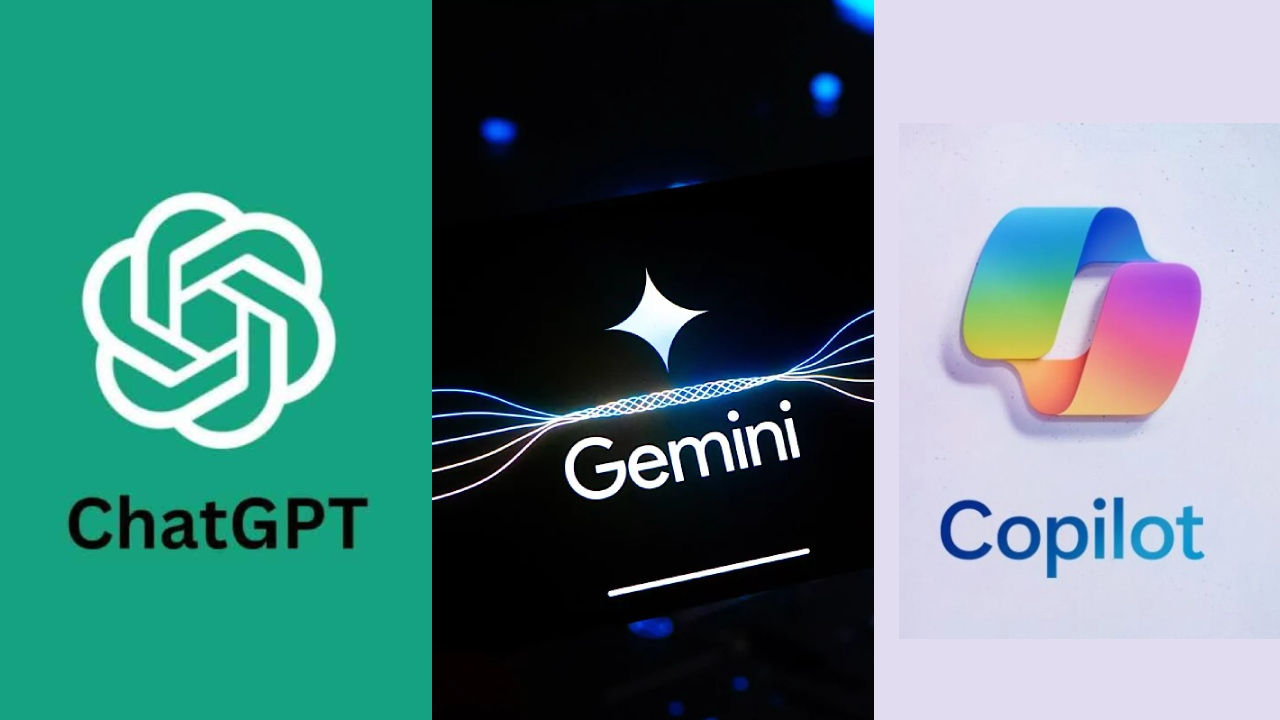
\includegraphics[width=1\linewidth]{imagenes/pdl.jpg}
    \caption[\textbf{Ejemplos de modelos generativos de lenguajes}.]{\textbf{Ejemplos de modelos generativos de lenguajes}. ChatGPT, Gemini y Copilot, tres de los LLMs más avanzados y reconocidos en la actualidad. \href{https://static1.srcdn.com/wordpress/wp-content/uploads/2024/01/tlou2r-joel-horse.JPG}{https://static1.srcdn.com/wordpress/wp-content/uploads/2024/01/tlou2r-joel-horse.JPG}}
    \label{modelos-generativos-de-lenguajes}
\end{figure}

\newpage

\subsection{LangChain}

La información que se presenta a continuación ha sido obtenida de la página web oficial de LangChain y un publicación de Vasilios Mavroudis.

LangChain es una tecnología que permite a las aplicaciones razonar y procesar información de manera más inteligente. Es utilizada por múltiples empresas de gran renombre, como Google y Rakuten TV. LangChain facilita la construcción de aplicaciones que integran LLMs, permitiendo que estas interactúen de forma dinámica y contextual con los usuarios.

Para cadenas y flujos de recuperación más sencillos, se recomienda usar LangChain junto con LangChain Expression Language para ensamblar componentes. Si estamos creando agentes o necesitamos una orquestación más compleja, utilizamos LangGraph.

Por otro lado, \textbf{LangGraph Platform} se encarga de la ejecución, permitiendo desplegar y ejecutar las aplicaciones de manera eficiente. Además, \textbf{LangSmith} ofrece herramientas para gestionar y probar las aplicaciones, asegurando su correcto funcionamiento y mejorando el rendimiento. \cite{PaginaLangChainOficial} \cite{mavroudis2024langchain}



\begin{figure}[H]
    \centering
    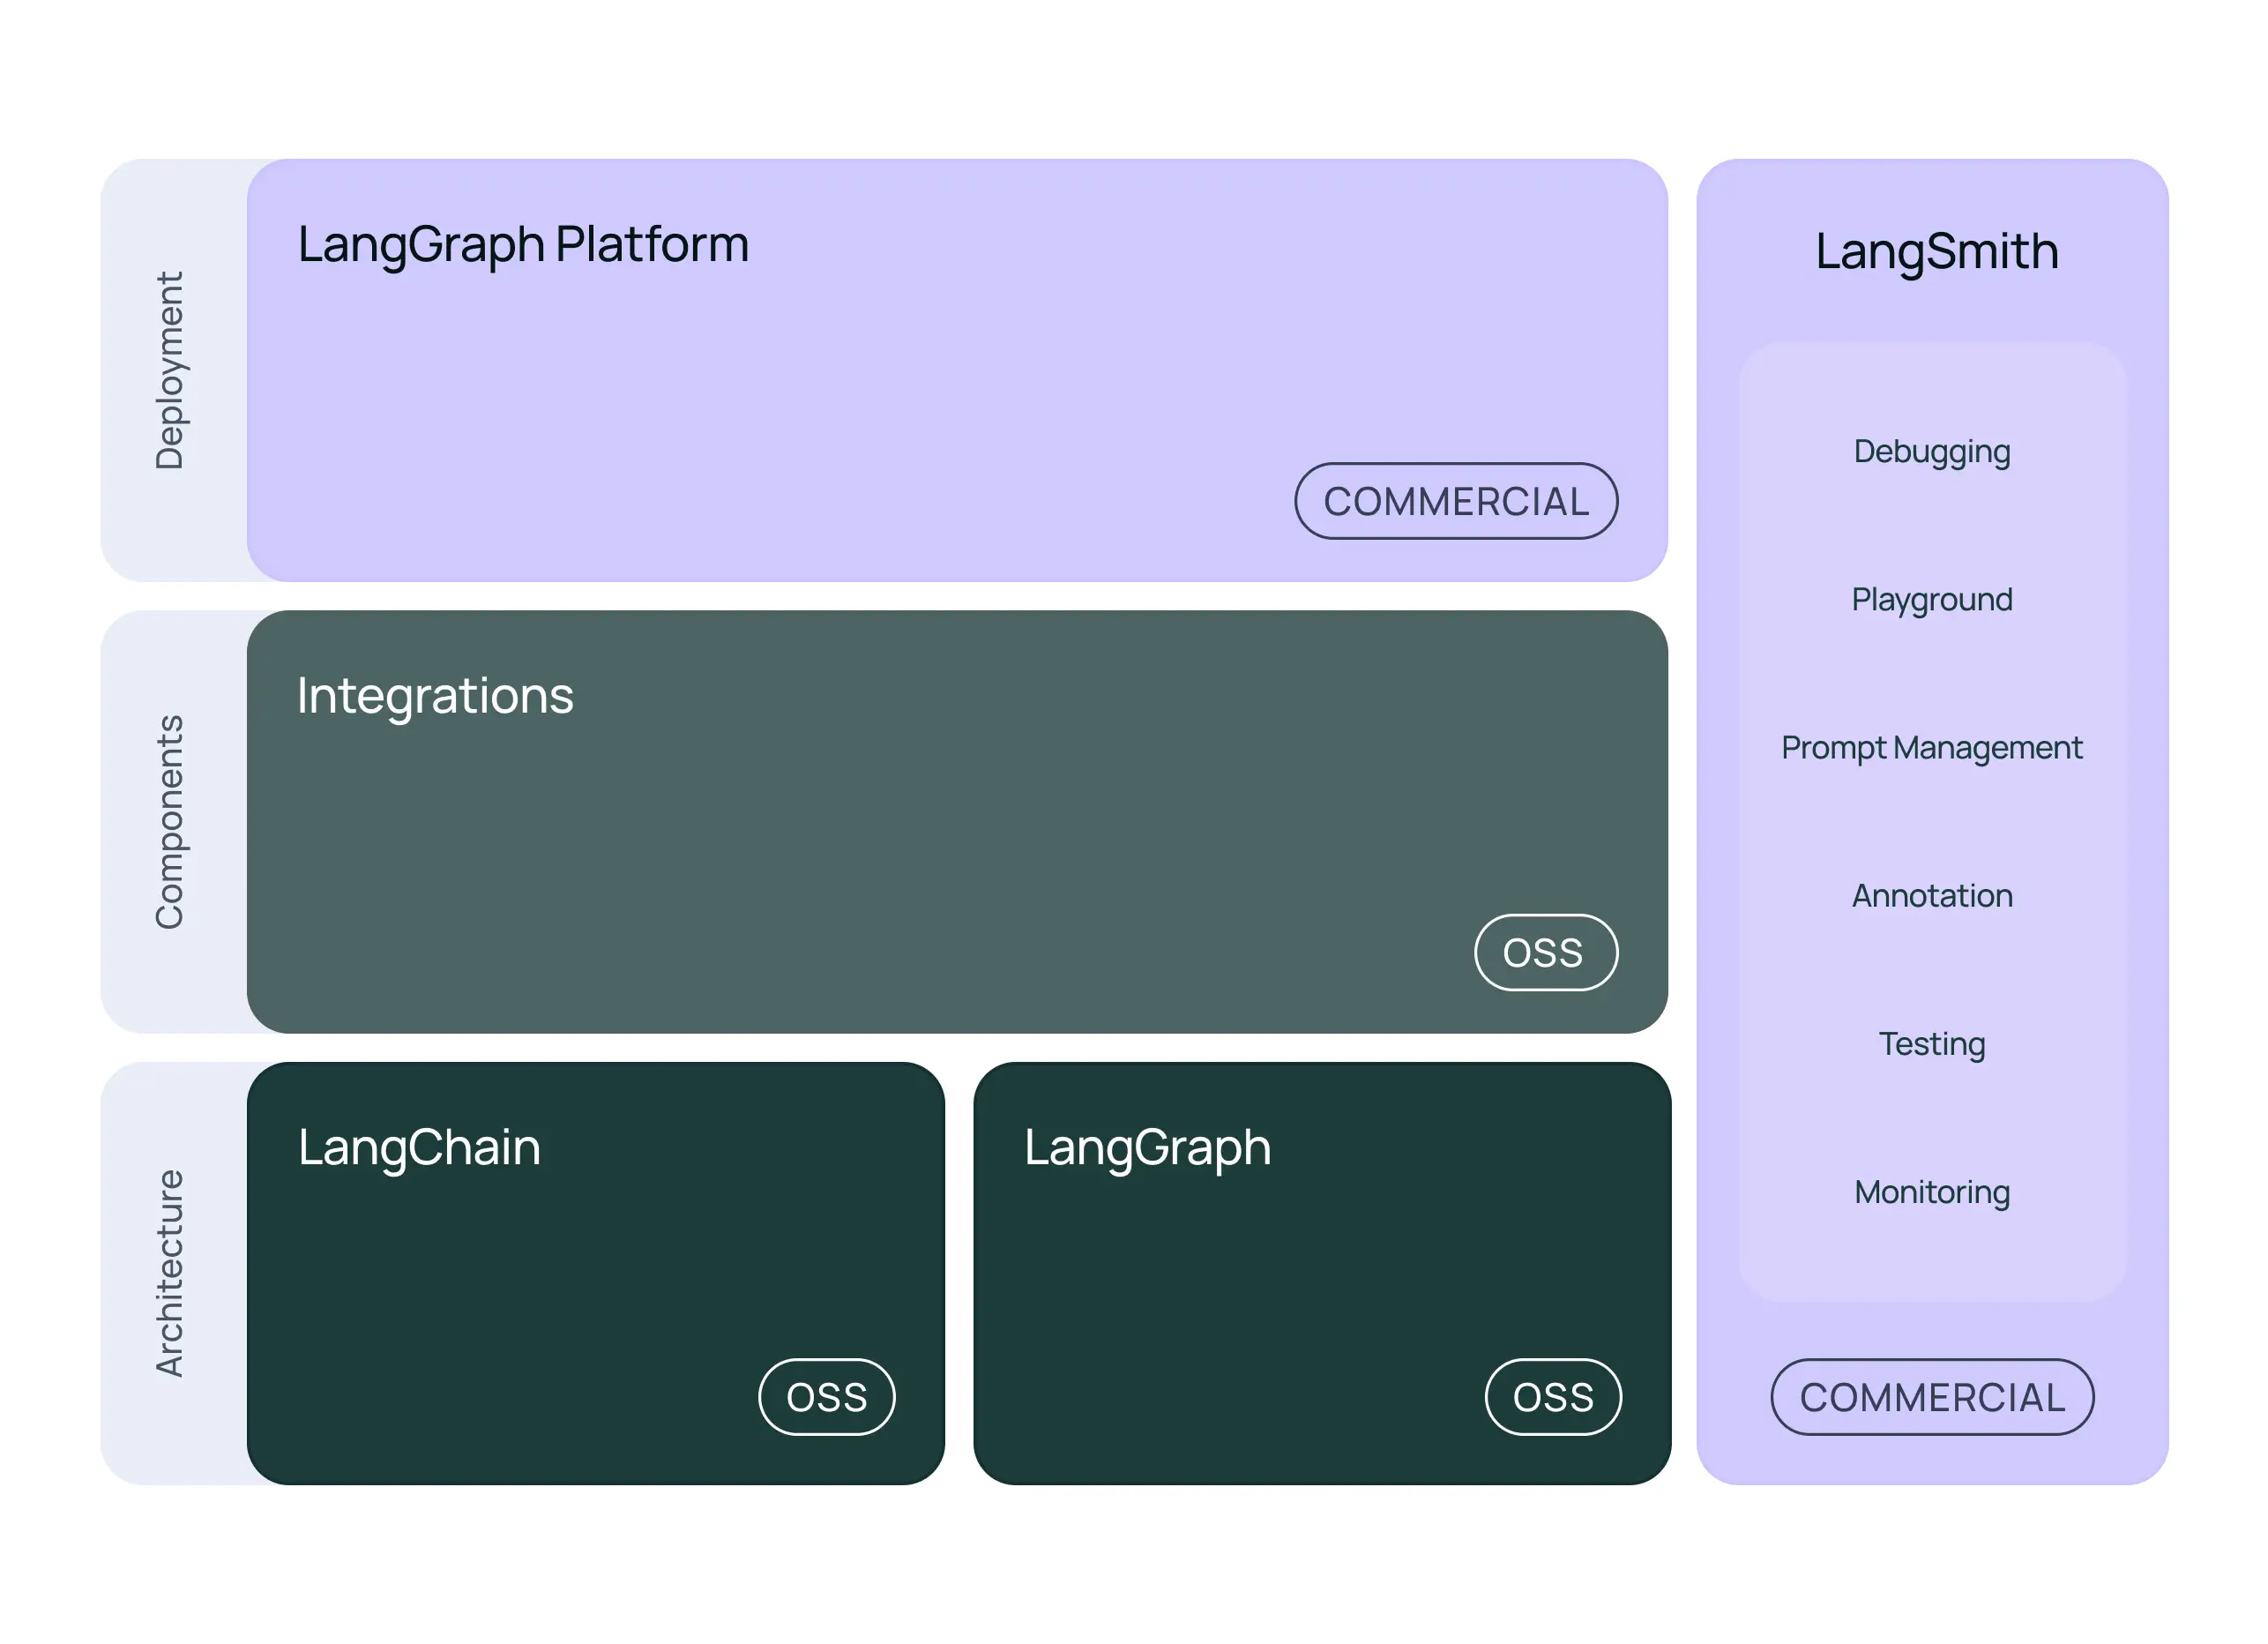
\includegraphics[width=\linewidth]{imagenes/lg.jpg}
    \caption[\textbf{Arquitectura productos LangChain}.]{\textbf{Arquitectura productos LangChain}. La arquitectura de referencia que las empresas adoptan para el éxito. Los productos de LangChain pueden usarse de forma independiente o combinada para lograr un impacto multiplicador, guiando en la construcción, ejecución y gestión de aplicaciones LLM. \cite{PaginaLangChainOficial}}
    \label{productos-lang-chain} 
\end{figure}


Procedamos a analizar cada producto por separado.


\subsubsection{LangChain básico}

Es la tecnología base de todos los productos. Es compatible con JavaScript y Python. Cuenta con una amplia biblioteca de componentes para usar de principio a fin en las aplicaciones. Conecta los modelos generativos de lenguajes con cualquier fuente de datos o conocimiento, y APIs para crear aplicaciones conscientes del contexto y con capacidad de razonamiento, utilizando métodos populares como RAG (Retrieval-Augmented Generation), que recupera la información del usuario de, por ejemplo, bases de datos antes de generar una respuesta, para mejorarla; y cadenas simples, en las que se solicita la pregunta al usuario, se pasa al LLM y se envía la respuesta al usuario. LangChain es fácil de comenzar a usar y ofrece elección, flexibilidad y potencia a medida que escalas. Cuenta con más de 3000 colaboradores, la comunidad más grande de cualquier framework centrado en LLM, más de 600 integraciones y es fácil de usar, pero robusto para producción. Además, es de código abierto. \cite{PaginaLangChainOficialBasico} \cite{mavroudis2024langchain}


\subsubsection{Métodos}

En LangChain, diversos métodos avanzados permiten optimizar la interacción con los modelos generativos de lenguajes, facilitando la integración de datos, la mejora en el procesamiento y la generación de respuestas. Estos métodos permiten adaptar el comportamiento del sistema a necesidades específicas, desde la recuperación de información relevante hasta la ejecución de tareas automatizadas mediante agentes. Vamos a explorar algunos de los métodos clave utilizados en LangChain, como la Generación Aumentada por Recuperación (RAG), los agentes inteligentes y las herramientas de evaluación de rendimiento, que son fundamentales para el desarrollo de aplicaciones inteligentes y contextualmente conscientes.

\textbf{RAG}

La \textbf{Generación Aumentada por Recuperación (RAG)} con LangChain y sus métodos integrados de gestión y recuperación conecta los datos con el poder de los LLMs. Dispone de herramientas de importación de documentos para cualquier tipo de datos.

Dispone de diversos algoritmos avanzados de recuperación, entre ellos:

\begin{itemize}
    \item \textbf{Time-Weighted Vector Store:} combina la similitud semántica con un decaimiento temporal para tener en cuenta la actualidad en las recuperaciones.
    \item \textbf{Parent Document Retriever:} incorpora fragmentos pequeños, que son mejores para la búsqueda por similitud, pero recupera fragmentos más grandes que ayudan en la generación de contenido.
    \item \textbf{Self Query Retriever:} analiza la consulta en lenguaje natural y escribe una consulta estructurada para ejecutarla en el VectorStore subyacente.
    \item \textbf{Contextual Compression:} comprime el documento recuperado utilizando el contexto de la consulta, de modo que únicamente se retiene la información relevante de la fuente.
    \item \textbf{Multi Vector Retriever:} realiza consultas en múltiples vectores almacenados por documento, incluidos fragmentos más pequeños, resúmenes y preguntas hipotéticas.
\end{itemize}

La API de indexación de LangChain sincroniza los datos desde cualquier fuente hacia un almacén vectorial, ayudándote a ahorrar tiempo y recursos. \cite{PaginaLangChainOficialRAG} \cite{mavroudis2024langchain}

\textbf{Agentes}

Los agentes pueden crear borradores iniciales para revisión a posteriori, actuar en tu nombre o esperar tu aprobación antes de la ejecución. LangGraph ofrece control para flujos de trabajo personalizados de agentes y multi-agentes, interacciones fluidas con intervención humana, y soporte nativo para transmisión de datos, lo que mejora la fiabilidad y ejecución de los agentes. Permite llamar de manera forzada a una herramienta, esperar la aprobación de intervención humana, la colaboración de múltiples agentes en un objetivo común y transmitir los pasos intermedios a medida que ocurren. Además, LangSmith ofrece la capacidad de explicar por qué los agentes se desvían y cómo hacer que vuelvan a funcionar correctamente. \cite{PaginaLangChainOficialAgentes} \cite{mavroudis2024langchain}

\textbf{Evaluación}

LangSmith permite medir el rendimiento de la aplicación a lo largo de todo su ciclo de desarrollo con multitud de métricas. Se puede usar evaluación offline, con integración continua y online.

Un marco de pruebas sólido comienza con la creación de un conjunto de datos de referencia, una tarea que a menudo resulta tediosa. LangSmith simplifica esto permitiéndote guardar las trazas de depuración y producción en conjuntos de datos. Los conjuntos de datos son colecciones de entradas y salidas ejemplares o problemáticas que deben ser replicadas o corregidas, respectivamente. También te permite hacer un seguimiento de cómo se comparan las diferentes versiones de tu aplicación según los criterios de evaluación que hayas definido. Además, facilita la evaluación humana y en línea, no solo latencia, errores y costos, sino también medidas cualitativas para asegurar que tu aplicación responda de manera efectiva y cumpla con las expectativas del usuario. \cite{PaginaLangChainOficialEvaluacion} \cite{mavroudis2024langchain}


 
\subsubsection{LangGraph}

LangGraph controla, modera y guía las acciones de los agentes, evitando que se desvíen del curso previsto. Permite diseñar flujos de control diversos, tales como simples, multi-agentes, jerárquicos o secuenciales, todo dentro de un único marco de trabajo. Además, tiene la capacidad de guardar los historiales de conversación y los datos de la sesión, lo que permite mantener el contexto a lo largo del tiempo y asegurar transferencias suaves de información, incluso hacia atrás.

LangGraph ofrece múltiples opciones de despliegue, incluye un estudio visual y es de código abierto, lo que facilita su integración y personalización.

Asimismo, cuenta con una plataforma diseñada para desplegar y escalar aplicaciones LangGraph, con una API orientada a la creación de interfaces de usuario (UX) para agentes, además de un entorno de desarrollo integrado. Sin embargo, a diferencia de su núcleo, esta plataforma no es de código abierto.\cite{PaginaLangChainOficialLangGraph} \cite{mavroudis2024langchain}


 

\subsubsection{LangSmith}

LangSmith es una plataforma todo en uno diseñada para desarrolladores, que abarca cada etapa del ciclo de vida de las aplicaciones impulsadas por modelos generativos de lenguajes, tanto si utilizan LangChain como si no.

Esta herramienta permite depurar, colaborar, realizar pruebas y monitorear, ofreciendo una visibilidad completa de toda la secuencia de llamadas. Esto facilita la identificación precisa de errores y cuellos de botella en el rendimiento en tiempo real. Además, permite revisar, etiquetar y evaluar el comportamiento de los agentes de forma sencilla, mejorando así la eficiencia y la fiabilidad del sistema.  

LangSmith también puede ejecutarse de forma local, proporcionando flexibilidad y control total sobre el entorno de desarrollo.  \cite{PaginaLangChainOficialLangSmith} \cite{mavroudis2024langchain}

\newpage
\section{Estado del arte}

La revisión de la literatura existente nos permite comprobar si ya se ha desarrollado un proyecto similar al nuestro, lo que puede servir como fuente de inspiración, guía o referencia para evaluar la novedad de nuestro trabajo.

Tras una exhaustiva búsqueda, no se ha encontrado ningún trabajo o artículo que aborde específicamente el uso de LangChain para la recomendación de videojuegos. Esto sugiere que nuestro proyecto podría ser innovador en este ámbito.

Sin embargo, en una búsqueda más general, se han identificado artículos relacionados que merecen ser destacados:

Un caso relevante es el de las \textbf{recomendaciones} en otros ámbitos \textbf{utilizando LangChain}. En un trabajo publicado por el Journal of Industrial Engineering and Applied Science, se observa cómo un grupo de estudiantes diseñó un sistema para recomendar anime de manera personalizada, utilizando LangChain. Los resultados obtenidos sometidos a numerosas métricas fueron muy satisfactorios gracias a las capacidades de esta tecnología. \cite{zhang2024unlocking}

Otro trabajo notable es el de Johans Quintero, quien desarrolló un sistema que recomienda recursos mediante mecanismos de Procesamiento de Lenguaje Natural, utilizando agentes de LangChain. Este proyecto se centra principalmente en la recomendación de libros, pero su enfoque podría extrapolarse a otros ámbitos. \cite{recommender-agent-langchain}

En cuanto a la \textbf{recomendación de videojuegos}, se han encontrado trabajos relevantes que utilizan otras tecnologías. Por ejemplo, Daniel Yélamos Pérez creó un sistema de recomendación de videojuegos basado en las opiniones de otros usuarios, empleando técnicas de extracción e interpretación semántica de datos en un entorno informal. \cite{yelamos2016recomendacion}

Por último, cabe mencionar el trabajo de Alejandro Roldán Soblechero, quien desarrolló una aplicación móvil que permite a los usuarios opinar sobre videojuegos. Esta aplicación integra datos de IGDB (Internet Game Database) y otras bases de conocimiento, garantizando la solidez y actualidad de las sugerencias generadas por el sistema de recomendación. \cite{roldan2024aplicacion}

La siguiente tabla resume las características principales de cada trabajo:

\begin{table}[H]
	\centering
	\caption{Comparativa entre trabajos analizados y el presente proyecto}
	\label{tab:comparativa-trabajos}
	\begin{tabular}{|p{5cm}|c|c|c|c|c|}
		\hline
		\textbf{Trabajo} & \textbf{C1} & \textbf{C2} & \textbf{C3} & \textbf{C4} & \textbf{C5} \\
		\hline
		\textit{Unlocking Personalized Anime Recommendations: Langchain and LLM at the Forefront} & \ding{51} & \ding{55} & \ding{51} & \ding{55} & \ding{51} \\
		\hline
		\textit{Sistema de recomendación con agente LangChain} & \ding{51} & \ding{55} & \ding{51} & \ding{55} & \ding{51} \\
		\hline
		\textit{Recomendación de videojuegos basado en análisis semántico y minería de opinión} & \ding{55} & \ding{51} & \ding{55} & \ding{55} & \ding{55} \\
		\hline
		\textit{Aplicación de recomendación de videojuegos (IGDB)} & \ding{55} & \ding{51} & \ding{51} & \ding{55} & \ding{55} \\
		\hline
		\textbf{Este trabajo} & \ding{51} & \ding{51} & \ding{51} & \ding{51} & \ding{51} \\
		\hline
	\end{tabular}
	
	\vspace{0.5cm}
	\textbf{Leyenda de columnas:}
	\begin{itemize}
		\item[C1] Uso de LangChain
		\item[C2] Dominio: Recomendación de videojuegos
		\item[C3] Uso de múltiples fuentes de datos
		\item[C4] Personalización contextual (recursos, accesibilidad, etc.)
		\item[C5] Implementación práctica con tecnologías actuales
	\end{itemize}
\end{table}


Estos estudios evidencian que tanto el ámbito de las recomendaciones de videojuegos como el uso de LangChain en sistemas de recomendación son temas explorados en la literatura, ofreciendo un valioso punto de referencia y posibles fuentes de inspiración. Sin embargo, la ausencia de trabajos que combinen específicamente LangChain con la recomendación de videojuegos destaca la originalidad y el carácter innovador de nuestro proyecto. 